\documentclass{article}
\usepackage{graphicx}
\graphicspath{ {/asay/Desktop/images/} }
\usepackage{color}
\usepackage{xcolor}
\usepackage{listings}
\usepackage{xepersian}
\usepackage{xstring}

\title{پاسخ تمرین شماره۳ درس طراحی پایگاه داده }
\author{امیر حسین عاصم یوسفی \\ ۹۶۱۱۰۳۲۳}
\setlatintextfont{Times New Roman}
\settextfont{B Nazanin}


\begin{document}
	\maketitle
	\section*{سوال ۱ } 
	
اگر دید خارجی که تعریف کردیم شامل کلید اصلی جدول مبنا باشد می توان اطلاعات بیشتری از جدول به دست آورد زیرا در این صورت می توان از روی اطلاعات جدول فیلد های محاسباتی تعریف کرد و کاربر می تواند با استفاده از جدول مبنا اطلاعات بیشتری به دست بیاورد . 
\\
فرض کنید می خواهیم سیستم یک اداره را طراحی کنیم و برای کارمندان بخش مالی یک دید از روی جدول اطلاعات کارمندان تعریف می کنیم حال  کاربر می تاوند اطلاعاتی از قبیل میانگین حقوق دریافتی و ... را  با یک بار فراخوانی از جدول مبنا به دست آورد و در دید خارجی تعریف شده ثبت کند 
\\
به این ترتیب کاربر  می تواند با کار کردن با دید خارجی اطلاعات بیشتری نسبت به جدول مبنا به دست آورد  . 
\hrule
\section*{سوال ۲}
با توجه به این که هر کلید کاندید می تواند یک ابر کلید باشد بنابراین زمانی که 
\lr{k}
ستون یک جدول کلید کاندید پس 
\textcolor{red}{\lr{k}}
ابر کلید برای این جدول داریم   . 
\hrule
\section*{سوال ۳}
\subsection*{\textcolor{red}{الف}}
با توجه به این که سوپر کلیدها باید یکتایی مقدار داشته باشند بنابراین سه سوپر کلید به شرح زیر می باشد  : 
\begin{center}
	\begin{enumerate}
		\item \lr{customerCellPhoneNumber}
		\item \lr{customerEmail}
		\item \lr{customerZipCode}
	\end{enumerate}
\end{center}
با توجه به این که هر زیر مجموعه از
\lr{H$_{R}$}
در صورتی که مینیمال باشد و یکتایی مقدار داشته باشد ، می تواند به عنوان کلید کاندید در نظر گرفته شود داریم  : 
\begin{center}
	\begin{enumerate}
		\item \lr{customerZipCode}
		\item \lr{(customerName , customerCellPhoneNumber)}
		\item \lr{customerEmail}
		\item \lr{customerAddress}
	\end{enumerate}
\end{center}
کلید های جایگیزین به صورت زیر می باشند   : 
\begin{center}
	\begin{enumerate}
		\item \lr{customerZipCode}
		\item \lr{customerEmail}
		\item \lr{customerAddress}
	\end{enumerate}
\end{center}
\subsection*{\textcolor{red}{ب}}
برای کلید اصلی 
\lr{customerZipCode}
 گزینه مناسبی می باشد . 
 
\subsection*{\textcolor{red}{ج}}
مزیت اضافه کردن این صفت می تواند در 
\lr{performance}
کوئری ها موثر باشد زیرا به جای این که یک مجموعه از صفات را برای شناسایی یک سطر استفاده کنیم ، به راحتی می توانم تنها با 
\lr{customerID}
یک مشتری و اطلاعات مربوط به آن را پیدا کنیم  . 
\\
از معایب اضافه کردن این صفت می تواند اضافه شدن جدول برای صفات چند مقداری باشد و از همه مهم تر درصورتی که ما داده ای وارد جدول کرده باشیم باید هزینه بسیار زیادی برای اضافه کردن این صفت پرداخت کنیم زیرا ایتدا باید ستونی با این عنوان به جدول اضافه کنیم و تک به تک با توجه به کلید اصلی قبلی مقدار 
\lr{customerID}
را به روزرسانی کنیم که بسیار بر عملکرد 
\lr{DBMS}
تاثیرگذار است . 
\hrule
\section*{سوال ۴}

با توجه به کلید های خارجی نمودار 
\lr{ER}
به شکل زیر می باشد  : 
\begin{center}
	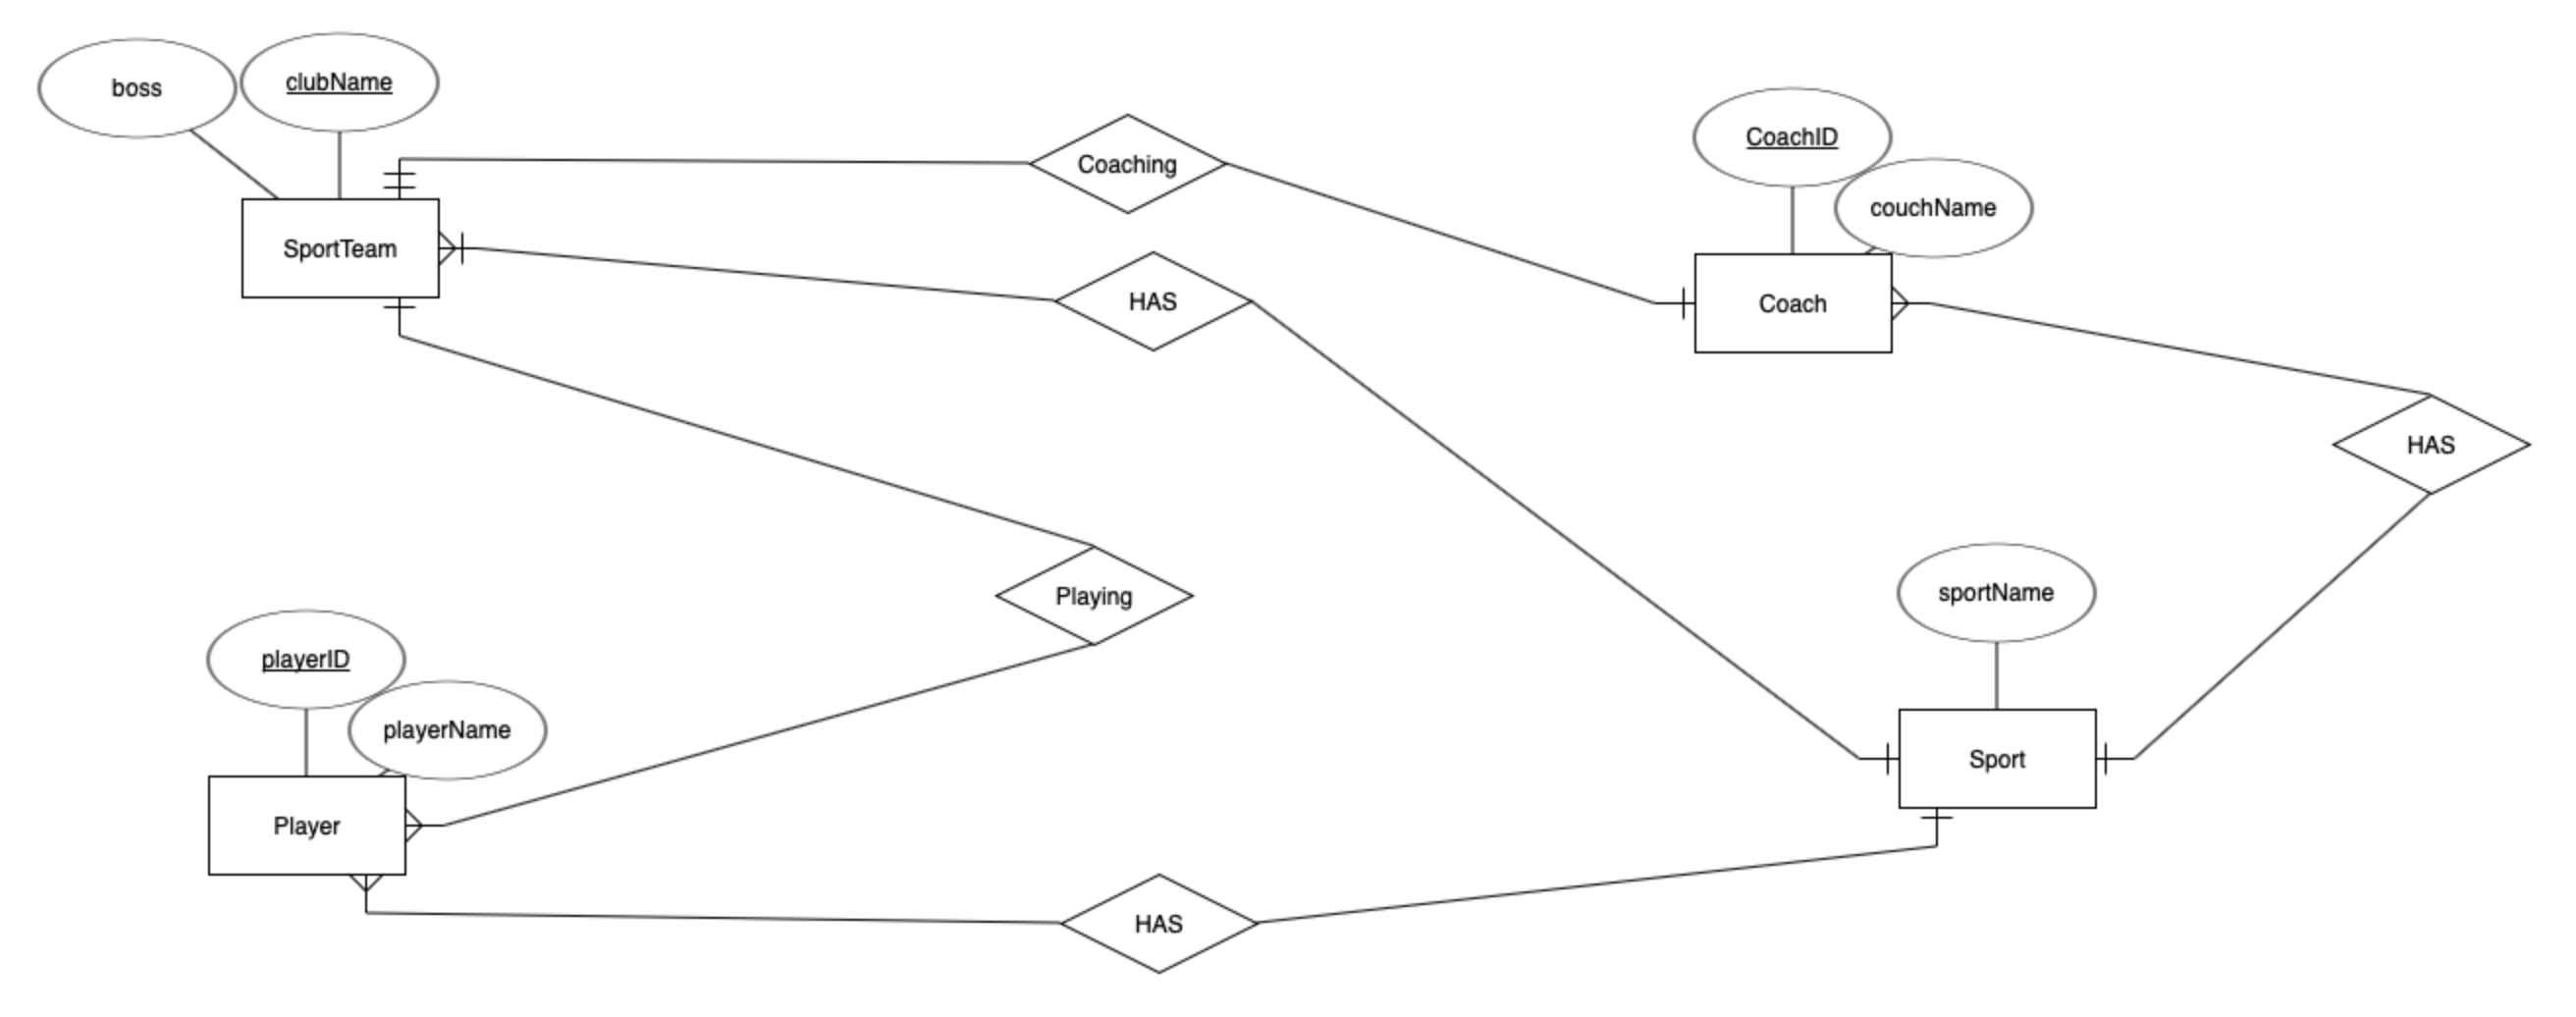
\includegraphics[width=1\textwidth]{ER}
\end{center}
با توجه به نمودار بالا گراف ارجاع به صورت زیر می باشد  : 
\begin{center}
	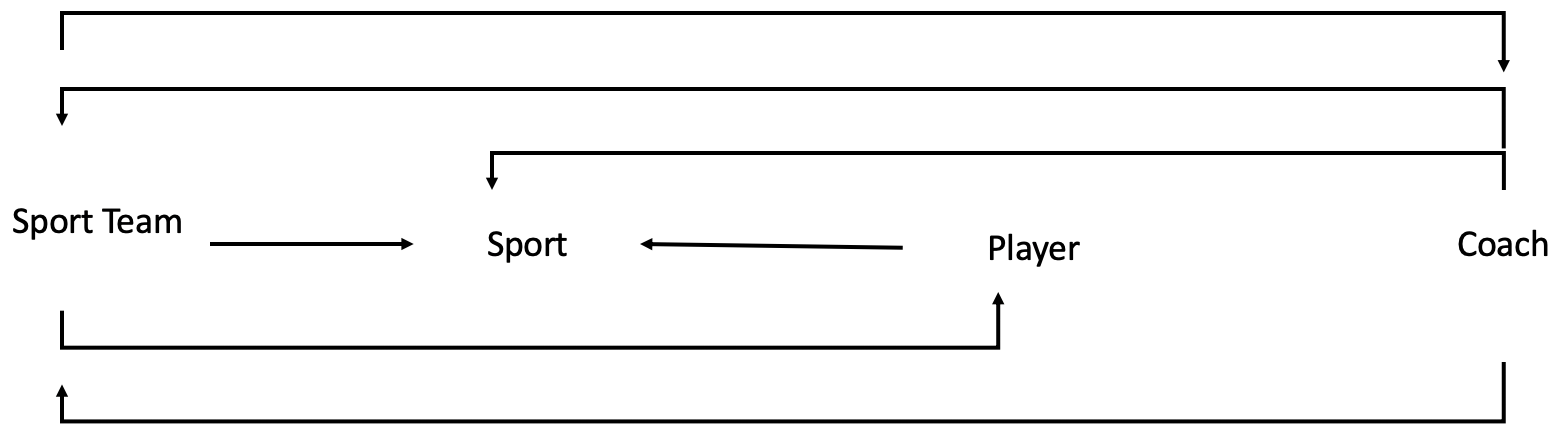
\includegraphics[width=1\textwidth]{graph}
\end{center}

\section*{سوال ۵}
\subsection*{\textcolor{red}{الف}}
\begin{flushleft}
\lr{Create View V1 as select * from Apply where Apply.StudentID in \\
(select stID from Sudent where studentID NOT IN \\
(select stID from Supervising));}
\newline
\newline
\lr{Create View V2 as select * from Student where studentID NOT IN \\
(select stID from Supervising);}
\newline
\newline
\lr{Create View Final as select * from V1 JOIN V2;}
\end{flushleft}

\subsection*{\textcolor{red}{ ب}}
\begin{flushleft}
	\lr{Create VIew V1 as select * from Student JOIN Department where ((Student.MotherTongue = Department.language) OR \\
		(Student.languageScore NOT NULL));
	 }
 \newline
\newline
\lr{Create View Final as select * from Student where StudetnID in \\
	(select studentID from V1);}
\end{flushleft}

\subsection*{\textcolor{red}{ج}}
\begin{flushleft}
	\lr{Create View Final as select * from Student where GPA in \\
		(select MAX(GPA) from Student where studentID in \\
		(select studentID from Apply where fieldName in \\
		(select DISTINCT (fieldName) from Apply)));}
\end{flushleft}

\hrule
\section*{سوال ۶}
پذیرا یا ناپذیرا بودن به شرح زیر می باشد  : 
\begin{center}
	\begin{enumerate}
		\item  ناپذیرا 
       \item 
       ناپذیرا
       \item پذیرا
       \item ناپذیرا
 \item پذیرا       
	\end{enumerate}

\end{center}
تبدیل
\lr{E/C}
برای شماره ۳ به صورت زیرا است  : 
\begin{flushleft}
	\lr{UPDATE Apply set fieldName= 'Data Mining' where fieldName = 'Data Science';}
\end{flushleft}
تبدیل 
\lr{E/C}
برای شماره ۵ به صورت زیر است  : 
\begin{flushleft}
	\lr{DELETE from Apply where fieldName = 'Computer Science';}
\end{flushleft}




\end{document}